\section{Dataset and Preprocessing}

The experiments are conducted on CIFAR-10~\cite{krizhevsky2009learning}, a standard image-classification benchmark consisting of ten object categories. 

\begin{figure}[H]
\centering
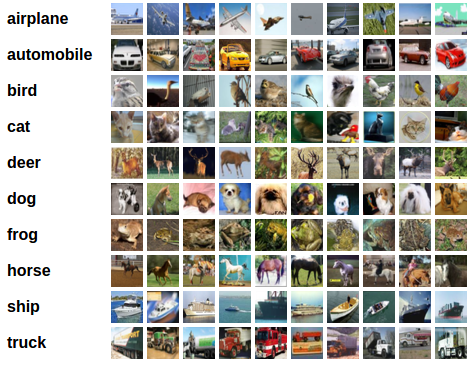
\includegraphics[width=0.72\linewidth]{figures/cifar10.png}
\caption[CIFAR-10 example images]{Example images from the CIFAR-10 dataset. CIFAR-10 contains ten object categories represented by low-resolution \(32 \times 32\) color images.}
\label{fig:ch5_cifar10_examples}
\end{figure}
Each image has spatial resolution \(32 \times 32\) with three color channels. The official dataset contains 50,000 training images and 10,000 test images. In our experimental pipeline, the original training split is partitioned into 40,000 images for training and 10,000 images for validation and checkpoint selection, while the official 10,000-image test split is reserved for final test-set evaluation.

The validation set is used only for model selection and hyperparameter monitoring. Final reported numbers are computed on the test set after the checkpoint has been selected. This separation is important because adversarial robustness estimates can vary across random seeds and training checkpoints; using a held-out validation set reduces the risk of selecting a checkpoint based on test-set performance.
All images are normalized using the same preprocessing pipeline across methods. During training, standard CIFAR-10 data augmentation is applied to the clean images before adversarial examples are generated. The augmentation includes random cropping with padding and random horizontal flipping. During validation and testing, no stochastic augmentation is used. This ensures that differences between methods are caused by the training objective rather than by differences in preprocessing or evaluation.

The same dataset split, preprocessing pipeline, and evaluation dataloaders are used for all compared methods. This includes the single-attack PGD-AT and DDN-AT baselines, Multi-AT, AttackDRO, Cluster-DRO, and AttackDRO++.
